% ============================================================
%  TESIS: Predicción del Riesgo País de Ecuador con ML y NLP
%  Universidad San Francisco de Quito — Maestría en Ciencia de Datos
% ============================================================
\documentclass[12pt, oneside]{report}

% --- Codificación y lenguaje ---
\usepackage[utf8]{inputenc}
\usepackage[T1]{fontenc}
\usepackage[spanish]{babel}

% --- Márgenes (APA / estilo USFQ) ---
\usepackage[left=3cm, right=2.5cm, top=3cm, bottom=3cm]{geometry}

% --- Tipografía ---
\usepackage{times}           % Times New Roman
\usepackage{setspace}
\doublespacing               % Doble espacio

% --- Matemáticas y símbolos ---
\usepackage{amsmath, amssymb}

% --- Tablas ---
\usepackage{booktabs}
\usepackage{longtable}
\usepackage{array}
\usepackage{multirow}
\usepackage{tabularx}

% --- Figuras ---
\usepackage{graphicx}
\usepackage{float}
\usepackage{caption}
\usepackage{subcaption}
\graphicspath{{figures/}{../notebooks/}}   % busca figuras en latex/figures/ y en notebooks/

% --- Colores y links ---
\usepackage[colorlinks=true, linkcolor=black, citecolor=black, urlcolor=blue]{hyperref}

% --- Bibliografía (APA 7) ---
\usepackage[style=apa, backend=biber, sortcites=true, sorting=nyt]{biblatex}
\addbibresource{referencias.bib}

% --- Código ---
\usepackage{listings}
\usepackage{xcolor}
\lstset{
    basicstyle=\small\ttfamily,
    backgroundcolor=\color{gray!10},
    frame=single,
    breaklines=true,
    captionpos=b
}

% --- Encabezado y pie de página ---
\usepackage{fancyhdr}
\pagestyle{fancy}
\fancyhf{}
\rhead{\thepage}
\lhead{\leftmark}
\renewcommand{\headrulewidth}{0.4pt}

% ============================================================
\begin{document}

% --- Portada ---
\begin{titlepage}
    \centering
    \vspace*{2cm}
    {\Large \textbf{Universidad San Francisco de Quito}\par}
    \vspace{0.5cm}
    {\large Colegio de Posgrados\par}
    {\large Maestría en Ciencia de Datos\par}
    \vspace{2cm}
    \rule{\textwidth}{1pt}\\[0.4cm]
    {\LARGE \textbf{Predicción del Riesgo País de Ecuador mediante Aprendizaje Automático e Información Mediática: Evidencia del EMBI 2013--2025}\par}
    \rule{\textwidth}{1pt}\\[2cm]
    {\large Daniel Plaza\par}
    \vspace{1cm}
    {\large Tesis de grado presentada como requisito para la obtención del título de\\ Magíster en Ciencia de Datos\par}
    \vspace{2cm}
    {\large Quito, Ecuador\par}
    {\large 2026\par}
\end{titlepage}

% --- Páginas preliminares con numeración romana ---
\pagenumbering{roman}
\setcounter{page}{2}

\chapter*{Resumen}
\addcontentsline{toc}{chapter}{Resumen}

% TODO: Escribir resumen en español (~250 palabras)
% Puntos a cubrir:
%   - Pregunta de investigación: ¿puede el ML + NLP predecir mejor el EMBI de Ecuador que métodos econométricos?
%   - Datos: 3.047 días de trading, 2013-2025, fuentes GDELT v2, Bloomberg/Yahoo Finance, macroeconomía local
%   - Métodos: ARIMA baseline, XGBoost con ablación, Granger, Chow/CUSUM, Autoencoder NLP
%   - Resultado principal: Grupo C (AR + NLP) alcanza RMSE 49.01 pb vs 107.48 pb del ARIMA (reducción 54.4%)
%   - Hallazgo exogeneidad: variables locales no mejoran el modelo; en crisis el desempleo local irrumpe
%   - Hallazgo NLP: la cobertura mediática (volumen) aporta señal; el sentimiento no
%   - Hallazgo autoencoder: la representación NLP es esencialmente lineal (PCA suficiente)

\vspace{1cm}

\noindent \textbf{Palabras clave:} riesgo país, EMBI, Ecuador, XGBoost, GDELT, NLP, quiebres estructurales, análisis de regímenes.

\vspace{1cm}

\chapter*{Abstract}
\addcontentsline{toc}{chapter}{Abstract}

% TODO: Traducir resumen al inglés

\vspace{1cm}

\noindent \textbf{Keywords:} country risk, EMBI, Ecuador, XGBoost, GDELT, NLP, structural breaks, regime analysis.


\tableofcontents
\listoffigures
\listoftables

% --- Cuerpo principal con numeración arábiga ---
\pagenumbering{arabic}
\setcounter{page}{1}

\chapter{Introducción}

% --------------------------------------------------------
\section{Contexto y motivación}
% --------------------------------------------------------
% TODO: ~500 palabras
% Puntos:
%   - El EMBI de Ecuador como indicador de riesgo soberano: qué mide, por qué importa
%   - Ecuador: economía dolarizada, historial de defaults (1999, 2008 Correa, 2020 pandemia)
%   - Costo económico: 1 pb en el EMBI representa decenas de millones USD en servicio de deuda
%   - Brecha: los modelos econométricos tradicionales (ARIMA) no capturan shocks exógenos ni información mediática
%   - Oportunidad: disponibilidad de datos GDELT v2 (noticias globales) + ML moderno

% --------------------------------------------------------
\section{Pregunta de investigación}
% --------------------------------------------------------
% TODO: ~200 palabras
% Pregunta principal: ¿Puede un modelo de aprendizaje automático entrenado con
%   variables macroeconómicas, financieras externas e información mediática (NLP)
%   predecir el EMBI de Ecuador con mayor precisión que el baseline ARIMA?
%
% Preguntas secundarias:
%   1. ¿Qué grupo de variables (AR, macro, NLP) contribuye más a la predicción?
%   2. ¿Anticipa el volumen de cobertura mediática los movimientos del EMBI (causalidad de Granger)?
%   3. ¿Existen quiebres estructurales que cambien qué variables determinan el EMBI?
%   4. ¿Mejora la compresión no lineal (autoencoder) la representación NLP?

% --------------------------------------------------------
\section{Objetivos}
% --------------------------------------------------------

\subsection{Objetivo general}
% TODO

\subsection{Objetivos específicos}
% TODO (4-5 objetivos alineados con las preguntas secundarias)

% --------------------------------------------------------
\section{Hipótesis}
% --------------------------------------------------------
% TODO:
%   H1: El XGBoost con variables AR + NLP supera al ARIMA en RMSE fuera de muestra
%   H2: El NLP aporta mejora incremental significativa sobre el modelo solo-AR
%   H3: No existe causalidad de Granger NLP → EMBI con rezago diario
%   H4: Existen quiebres estructurales estadísticamente significativos en 2020 y 2022

% --------------------------------------------------------
\section{Contribuciones}
% --------------------------------------------------------
% TODO: ~300 palabras
% 1. Primera aplicación sistemática de GDELT v2 para predicción del EMBI ecuatoriano
% 2. Experimento de ablación que aísla la contribución del NLP vs macro vs AR
% 3. Análisis de regímenes (Chow + CUSUM + SHAP) que muestra heterogeneidad estructural
% 4. Evidencia empírica sobre exogeneidad del EMBI ecuatoriano en períodos normales vs crisis

% --------------------------------------------------------
\section{Estructura del documento}
% --------------------------------------------------------
% TODO: párrafo breve describiendo cada capítulo

\chapter{Marco Teórico y Revisión de Literatura}

% --------------------------------------------------------
\section{El riesgo soberano y el EMBI}
% --------------------------------------------------------
% TODO: ~600 palabras
% - Definición del EMBI (Emerging Market Bond Index) — JP Morgan
% - Componentes: spread sobre US Treasury, qué mide
% - Determinantes teóricos: fundamentos fiscales, liquidez externa, apetito de riesgo global
% - Literatura sobre determinantes del riesgo soberano en América Latina
% - Especificidades de Ecuador: dolarización, ciclo del petróleo, historial crediticio

% --------------------------------------------------------
\section{Modelos econométricos para series financieras}
% --------------------------------------------------------
% TODO: ~400 palabras
% - ARIMA y familia ARIMA: ventajas y limitaciones para datos financieros
% - Stationarity, unit roots, ADF test
% - Por qué ARIMA falla en presencia de shocks exógenos y quiebres estructurales

% --------------------------------------------------------
\section{Aprendizaje automático para predicción financiera}
% --------------------------------------------------------
% TODO: ~500 palabras
% - XGBoost: gradient boosting, ventajas para datos tabulares con dependencias no lineales
% - Random Forest como comparador
% - Importancia de la validación temporal en series de tiempo (TimeSeriesSplit)
% - Literatura reciente: ML para spreads soberanos, CDS, bonos EM

% --------------------------------------------------------
\section{NLP y datos de noticias en economía financiera}
% --------------------------------------------------------
% TODO: ~500 palabras
% - GDELT: descripción del proyecto, cobertura global, variables disponibles
% - Antecedentes de uso de GDELT en economía: volatilidad, riesgo político, sentimiento
% - Hipótesis de eficiencia de mercado y relación con medios: ¿anticipan o reaccionan?
% - Distinción entre señal de volumen vs señal de sentimiento en mercados emergentes

% --------------------------------------------------------
\section{Causalidad de Granger en series financieras}
% --------------------------------------------------------
% TODO: ~300 palabras
% - Definición formal de causalidad de Granger
% - Aplicaciones en finanzas: noticias → mercados
% - Limitaciones: causalidad lineal, sensibilidad al lag elegido

% --------------------------------------------------------
\section{Análisis de quiebres estructurales}
% --------------------------------------------------------
% TODO: ~300 palabras
% - Test de Chow: hipótesis, supuestos, interpretación
% - Quandt-Andrews: quiebre óptimo sin fecha preimpuesta
% - CUSUM: inestabilidad acumulada de residuos
% - Literatura sobre regímenes en economías emergentes post-COVID

% --------------------------------------------------------
\section{Autoencoders para reducción de dimensionalidad}
% --------------------------------------------------------
% TODO: ~300 palabras
% - Arquitectura autoencoder: encoder, cuello de botella, decoder
% - Comparación con PCA (lineal) — cuándo la no-linealidad aporta
% - Aplicaciones en finanzas: representación de datos de mercado

\chapter{Datos y Metodología}

% --------------------------------------------------------
\section{Fuentes de datos}
% --------------------------------------------------------

\subsection{Variable objetivo: EMBI Ecuador}
% TODO: descripción de la serie, fuente, período 2004-2025, por qué se usa desde 2013

\subsection{Variables financieras externas}
% TODO: WTI, Gold, VIX, DXY, US Treasury 10Y, ETF EMB, ETF HYG — fuentes y justificación

\subsection{Variables macroeconómicas locales}
% TODO: reservas, balanza comercial, desempleo, liquidez M2 — frecuencia, fuente BCE/BM

\subsection{Datos NLP: GDELT v2}
% TODO: descripción de las 10 variables, filtro por mención a Ecuador, período desde sep-2013

% --------------------------------------------------------
\section{Preprocesamiento y construcción del dataset}
% --------------------------------------------------------

\subsection{Integración y alineación temporal}
% TODO: 3.047 días de trading, decisiones sobre NaN (exclusión de remesas y producción petrolera)

\subsection{División temporal del dataset}
% TODO: split 80/10/10 cronológico — justificación de no usar K-fold aleatorio
% Tabla: Train 2.406 días (2013-2024) | Val 274 días | Test 274 días

\subsection{Feature engineering}
% TODO: lags 1, 7, 30 días + rolling means 7 y 30 días → 132 features
% target_future = EMBI[t+1] como variable objetivo

\subsection{Selección de variables}
% TODO: Mutual Information sobre train exclusivamente → 60 variables seleccionadas
% Tabla de composición: 29 externas, 21 macro, 6 AR, 4 NLP

% --------------------------------------------------------
\section{Modelos y experimentos}
% --------------------------------------------------------

\subsection{Baseline: ARIMA}
% TODO: ARIMA(2,0,1) — selección por auto\_arima, validación rolling (ventana 3 años)

\subsection{XGBoost y Random Forest}
% TODO: RandomizedSearchCV, 100 iteraciones, TimeSeriesSplit 10 folds
% Hiperparámetros óptimos XGBoost (tabla)
% Wilcoxon Signed-Rank para comparar modelos

\subsection{Experimento de ablación}
% TODO: 4 grupos (A: AR, B: AR+Macro, C: AR+NLP, D: AR+Macro+NLP)
% Justificación: aislar contribución incremental de cada grupo de variables

\subsection{Causalidad de Granger}
% TODO: test sobre 4 variables NLP seleccionadas + avg\_tone + goldstein, lags 1-10

\subsection{Análisis de regímenes estructurales}
% TODO: Test de Chow (2020-03 y 2022-01), Quandt-Andrews, CUSUM, SHAP por subperiodo

\subsection{Autoencoder NLP}
% TODO: arquitectura 10→5→3→5→10, EarlyStopping, comparativa PCA-3 vs AE-3 vs original-4

% --------------------------------------------------------
\section{Métricas de evaluación}
% --------------------------------------------------------
% TODO: RMSE, MAE, R² — justificación de RMSE como métrica principal
% Nota sobre por qué el RMSE test es más relevante que el RMSE CV dado el alto std

\chapter{Resultados}

% --------------------------------------------------------
\section{Baseline ARIMA}
% --------------------------------------------------------

El modelo ARIMA(2,0,1), seleccionado automáticamente mediante criterio AIC, establece el piso de comparación.
La prueba ADF sobre el EMBI arroja estadístico $-4.336$ ($p = 0.0004$), confirmando estacionariedad en niveles.

\begin{table}[H]
\centering
\caption{Desempeño del baseline ARIMA}
\label{tab:arima}
\begin{tabular}{lcc}
\toprule
\textbf{Período} & \textbf{Esquema} & \textbf{RMSE (pb)} \\
\midrule
Validación & Rolling window (3 años) & 59.47 \\
Test        & Rolling window (3 años) & 107.48 \\
\bottomrule
\end{tabular}
\end{table}

% TODO: comentar el salto validación→test como evidencia de que ARIMA no captura shocks exógenos

% --------------------------------------------------------
\section{Selección de modelo ML: XGBoost vs Random Forest}
% --------------------------------------------------------

\begin{table}[H]
\centering
\caption{Comparación XGBoost vs Random Forest (CV, 10 folds)}
\label{tab:cv_comparison}
\begin{tabular}{lccc}
\toprule
\textbf{Modelo} & \textbf{RMSE CV medio (pb)} & \textbf{Std CV (pb)} & \textbf{p-valor Wilcoxon} \\
\midrule
Random Forest & 299.29 & $\pm$494.57 & \multirow{2}{*}{0.0273} \\
XGBoost       & 241.55 & $\pm$499.00 & \\
\bottomrule
\end{tabular}
\end{table}

% TODO: comentar el alto std como característica del EMBI ecuatoriano con picos extremos

Los hiperparámetros óptimos del XGBoost son: \texttt{n\_estimators=607}, \texttt{learning\_rate=0.093},
\texttt{max\_depth=4}, \texttt{subsample=0.848}, \texttt{colsample\_bytree=0.980},
\texttt{reg\_alpha=0.662}, \texttt{reg\_lambda=1.459}, \texttt{gamma=0.735}.

% --------------------------------------------------------
\section{Desempeño en test: XGBoost completo}
% --------------------------------------------------------

\begin{table}[H]
\centering
\caption{Métricas del XGBoost completo en test}
\label{tab:xgb_test}
\begin{tabular}{lc}
\toprule
\textbf{Métrica} & \textbf{Valor} \\
\midrule
RMSE  & 64.16 pb \\
MAE   & 34.90 pb \\
R$^2$ & 0.9555   \\
Mejora vs ARIMA & $-$40.3\% \\
\bottomrule
\end{tabular}
\end{table}

% --------------------------------------------------------
\section{Experimento de ablación}
% --------------------------------------------------------

% TODO: introducir los 4 grupos y su justificación

\begin{table}[H]
\centering
\caption{Resultados del experimento de ablación por grupo de variables}
\label{tab:ablation}
\begin{tabular}{lcccc}
\toprule
\textbf{Grupo} & \textbf{Features NLP} & \textbf{RMSE (pb)} & \textbf{MAE (pb)} & \textbf{R$^2$} \\
\midrule
ARIMA baseline      & ---  & 107.48 & ---   & ---    \\
A — Solo AR         & 0    & 51.31  & 27.15 & 0.9715 \\
B — AR + Macro      & 0    & 60.07  & 41.12 & 0.9610 \\
C — AR + NLP        & 4    & \textbf{49.01}  & \textbf{24.93} & \textbf{0.9740} \\
D — AR + Macro + NLP& 4    & 57.48  & 37.70 & 0.9643 \\
\bottomrule
\end{tabular}
\end{table}

% TODO: comentar hallazgos principales:
%   1. Grupo B peor que Grupo A — variables macro locales generan ruido
%   2. Grupo C mejor — NLP añade señal complementaria a los lags AR
%   3. Grupo D no es el mejor — combinación macro+NLP diluye el beneficio del NLP

% Wilcoxon tests
% TODO: reportar p-valores (A vs C: 0.1250, B vs D: 0.3125) y discutir bajo poder con 5 folds

% Figuras SHAP
\begin{figure}[H]
\centering
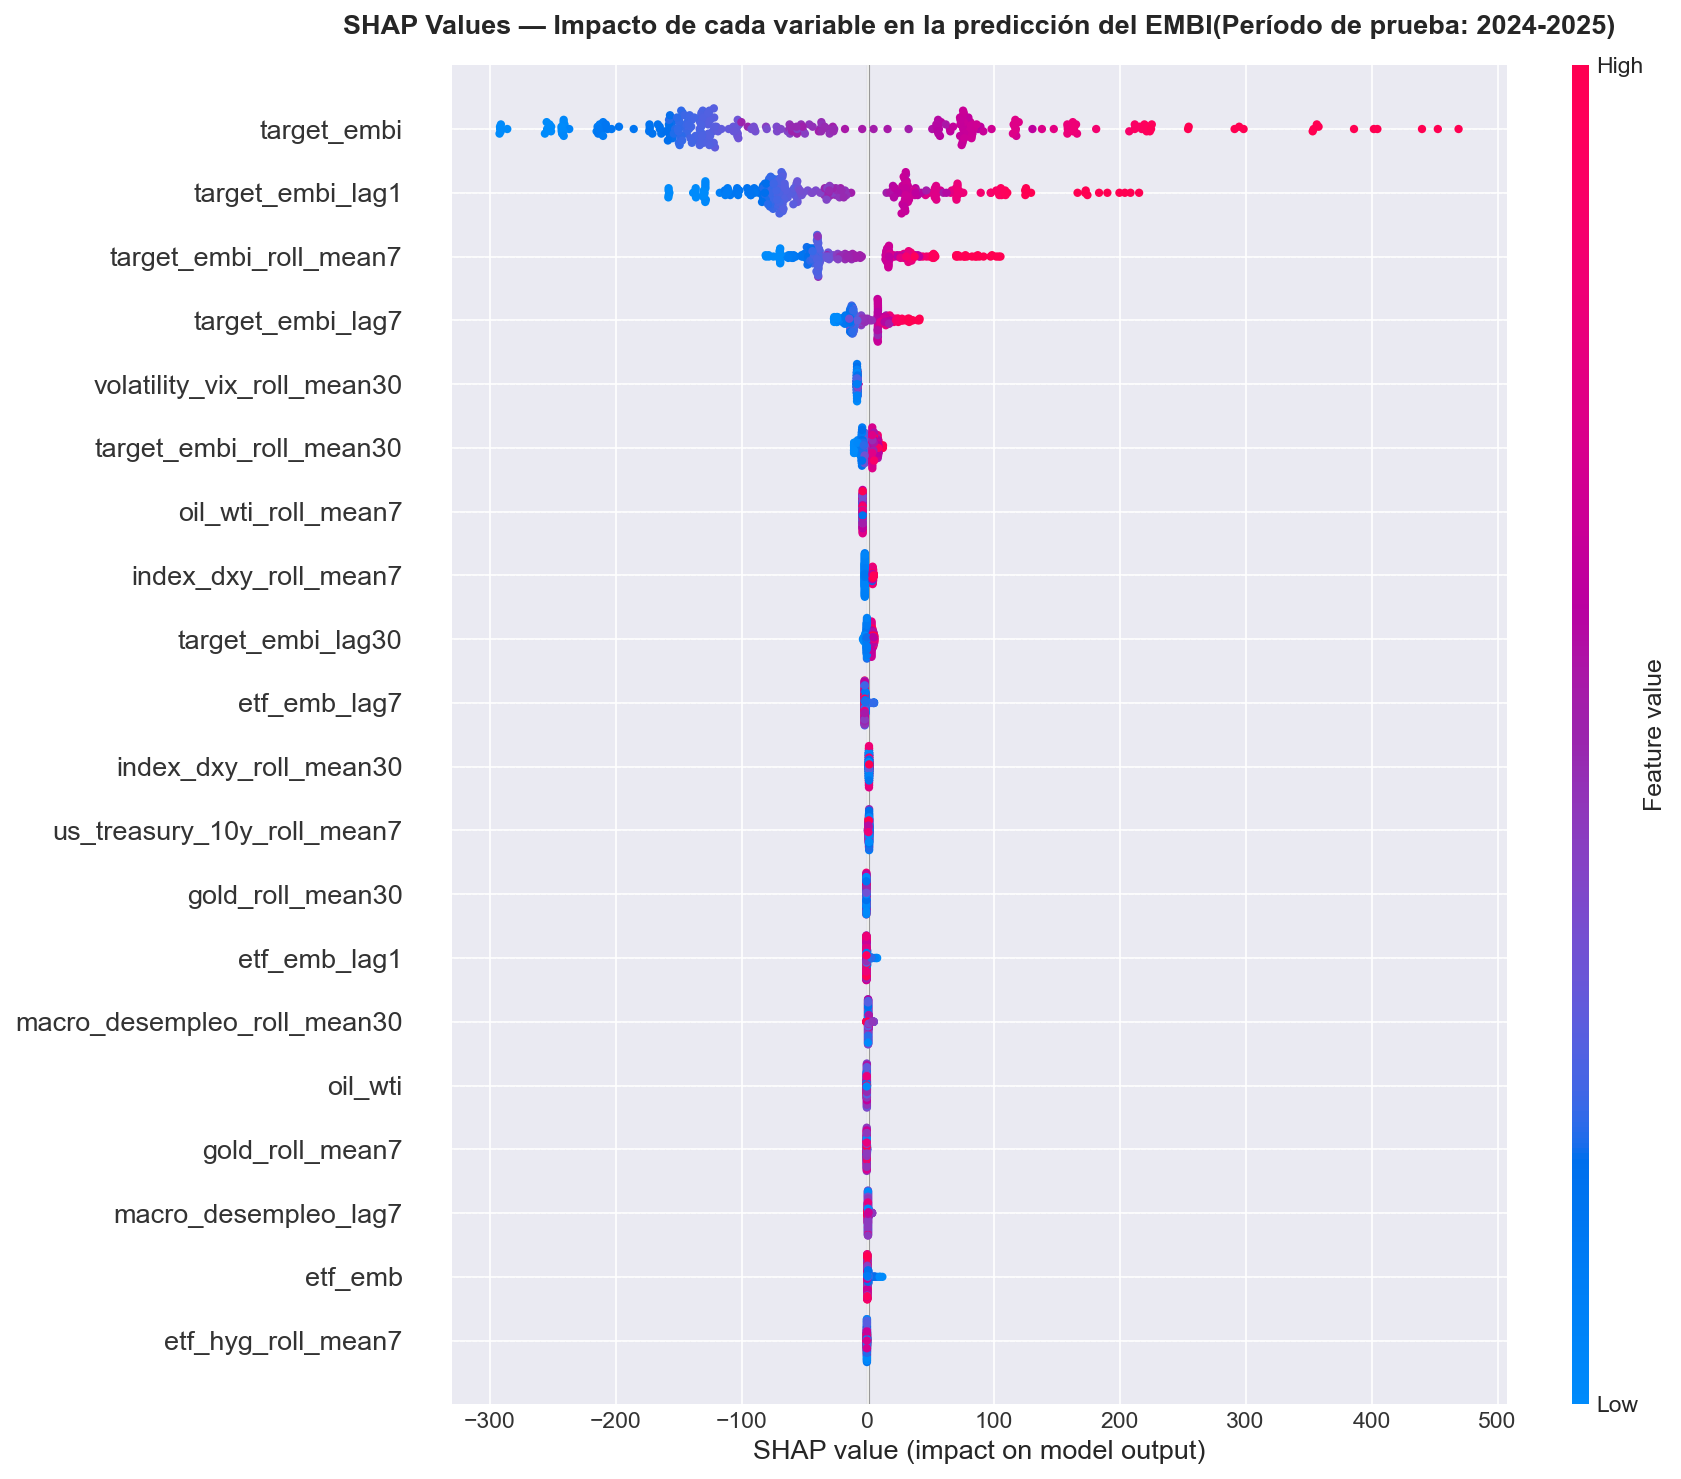
\includegraphics[width=0.85\textwidth]{shap_beeswarm.png}
\caption{SHAP beeswarm — importancia y dirección de las features en el modelo completo}
\label{fig:shap_beeswarm}
\end{figure}

\begin{figure}[H]
\centering
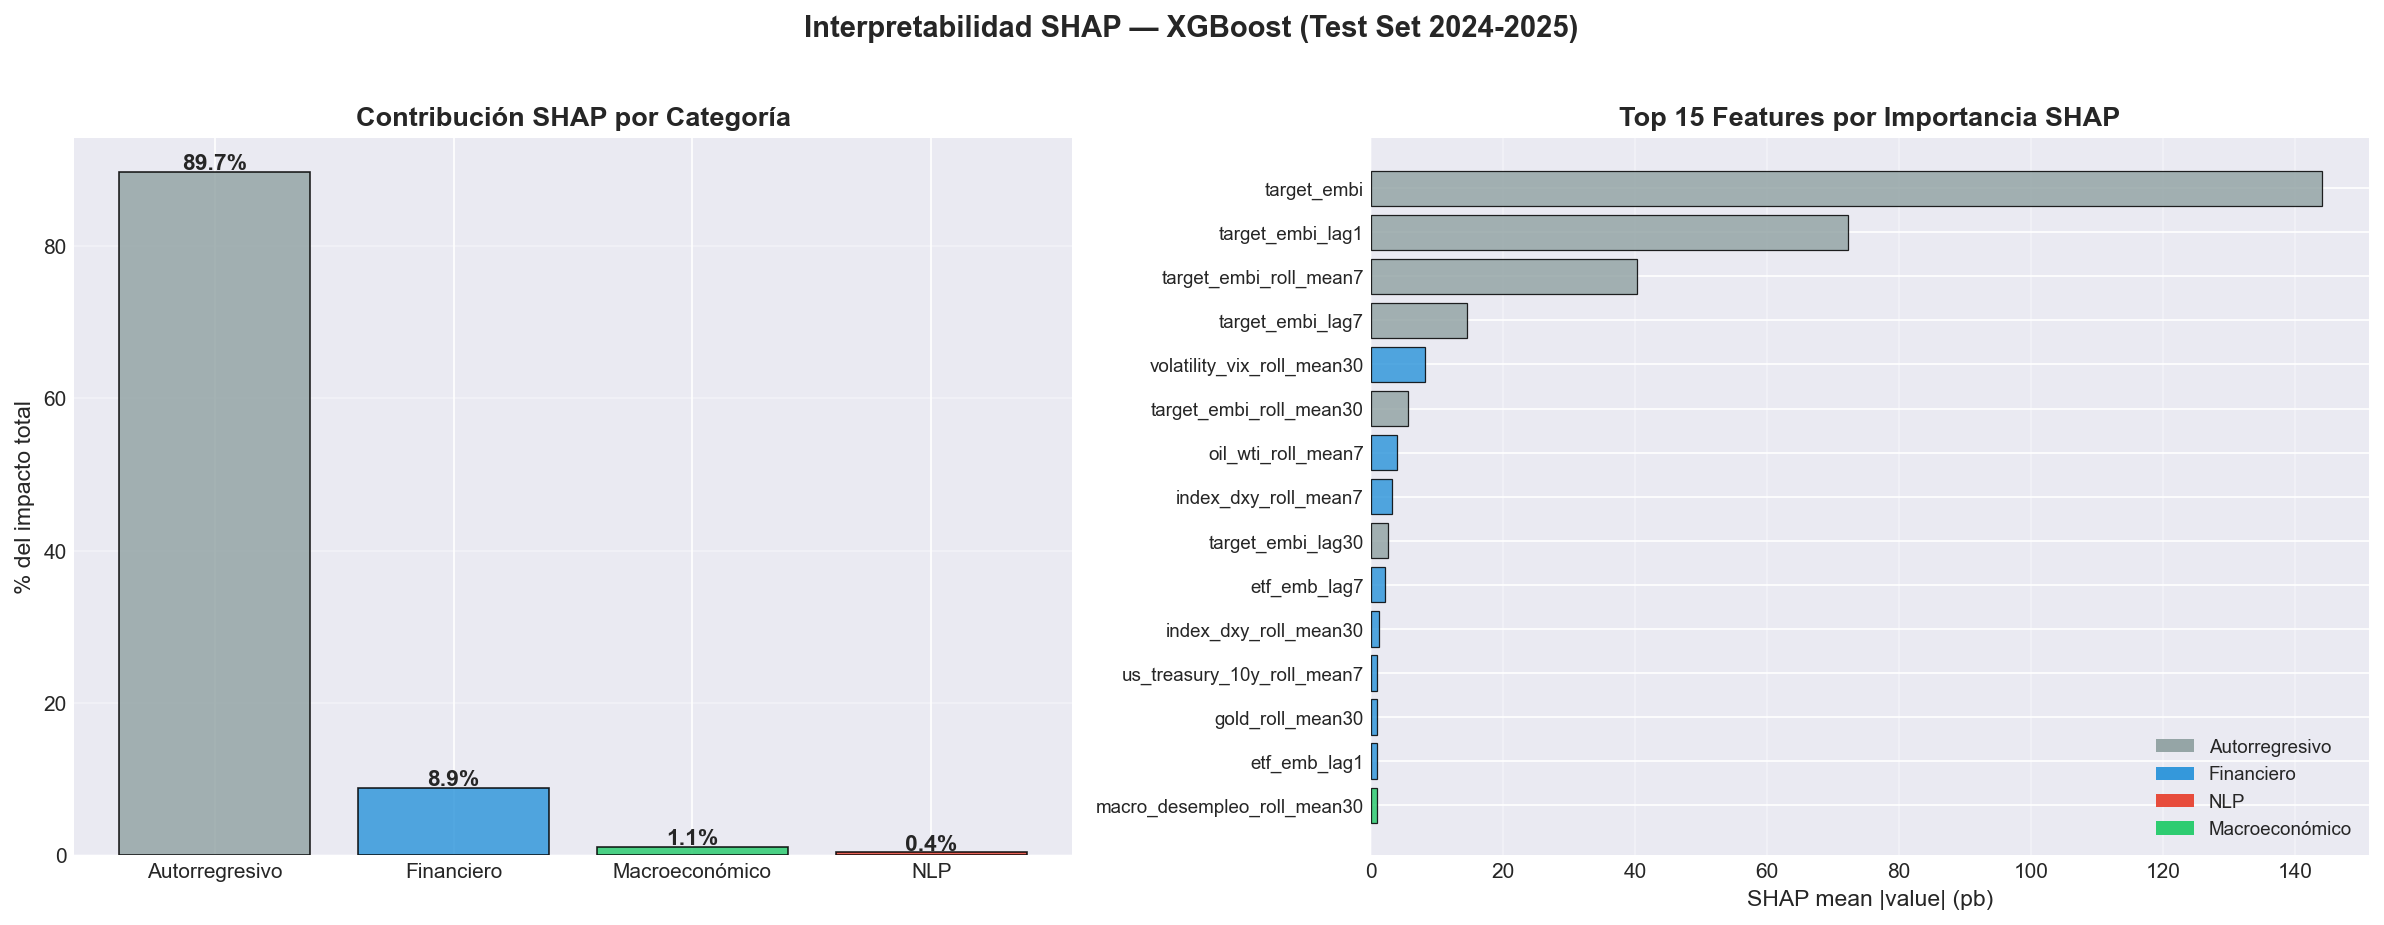
\includegraphics[width=0.85\textwidth]{shap_categorias.png}
\caption{Importancia SHAP agregada por categoría de variable}
\label{fig:shap_categorias}
\end{figure}

% --------------------------------------------------------
\section{Causalidad de Granger}
% --------------------------------------------------------

% TODO: tabla de resultados Granger (dirección, p-valor, lags significativos)
% Figura
\begin{figure}[H]
\centering
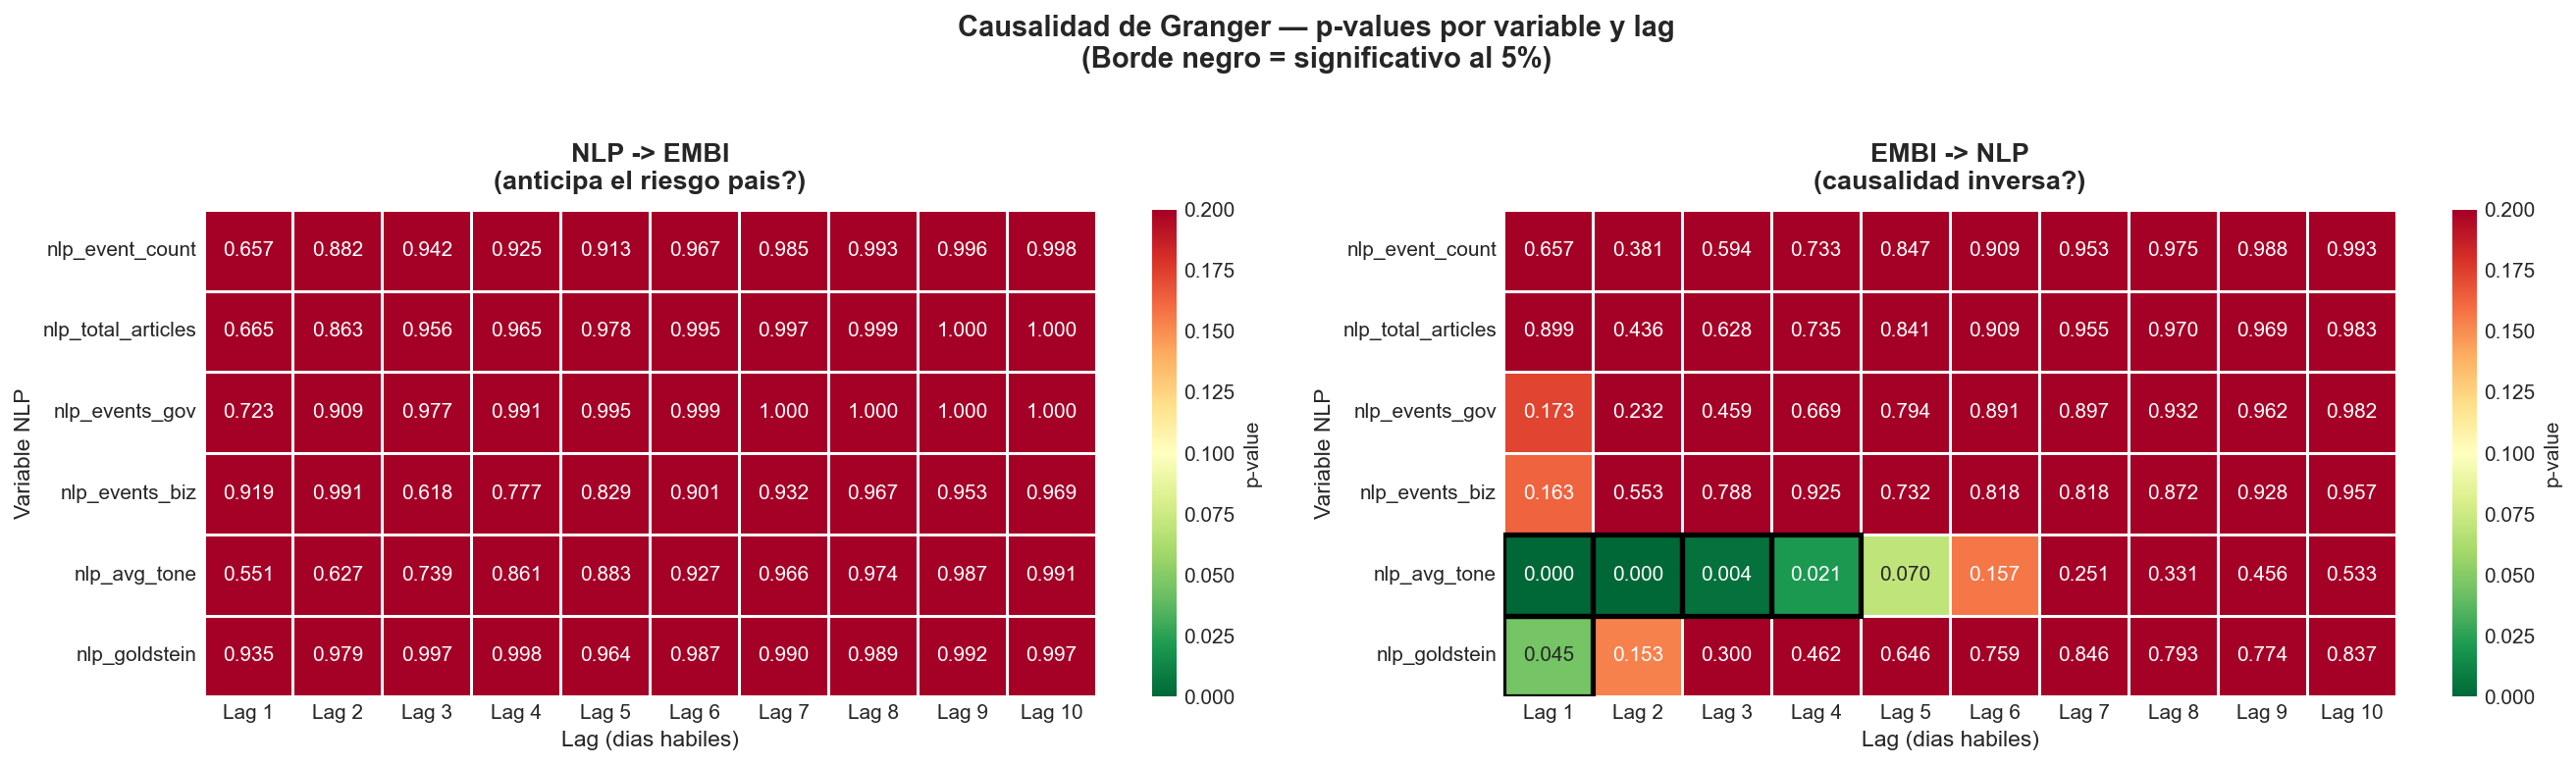
\includegraphics[width=0.75\textwidth]{granger_heatmap.png}
\caption{Heatmap de causalidad de Granger (lags 1--10 días hábiles)}
\label{fig:granger}
\end{figure}

% TODO: comentar: sin causalidad NLP→EMBI; causalidad inversa EMBI→tono (lags 1-4)

% --------------------------------------------------------
\section{Análisis de regímenes estructurales}
% --------------------------------------------------------

\subsection{Tests de quiebre estructural}

\begin{table}[H]
\centering
\caption{Resultados de los tests de quiebre estructural}
\label{tab:chow}
\begin{tabular}{lccccc}
\toprule
\textbf{Test} & \textbf{Fecha} & \textbf{F-stat} & \textbf{p-valor} & \textbf{n$_1$} & \textbf{n$_2$} \\
\midrule
Chow  & 2020-03-01 & 5.52  & 0.0002 & 1.587 & 1.457 \\
Chow  & 2022-01-01 & 11.61 & 0.0000 & 2.048 & 996   \\
Quandt-Andrews & 2020-03-25 & 53.58 & 0.0000 & --- & --- \\
CUSUM & --- & 0.848 & 0.469 & \multicolumn{2}{c}{No significativo} \\
\bottomrule
\end{tabular}
\end{table}

\begin{figure}[H]
\centering
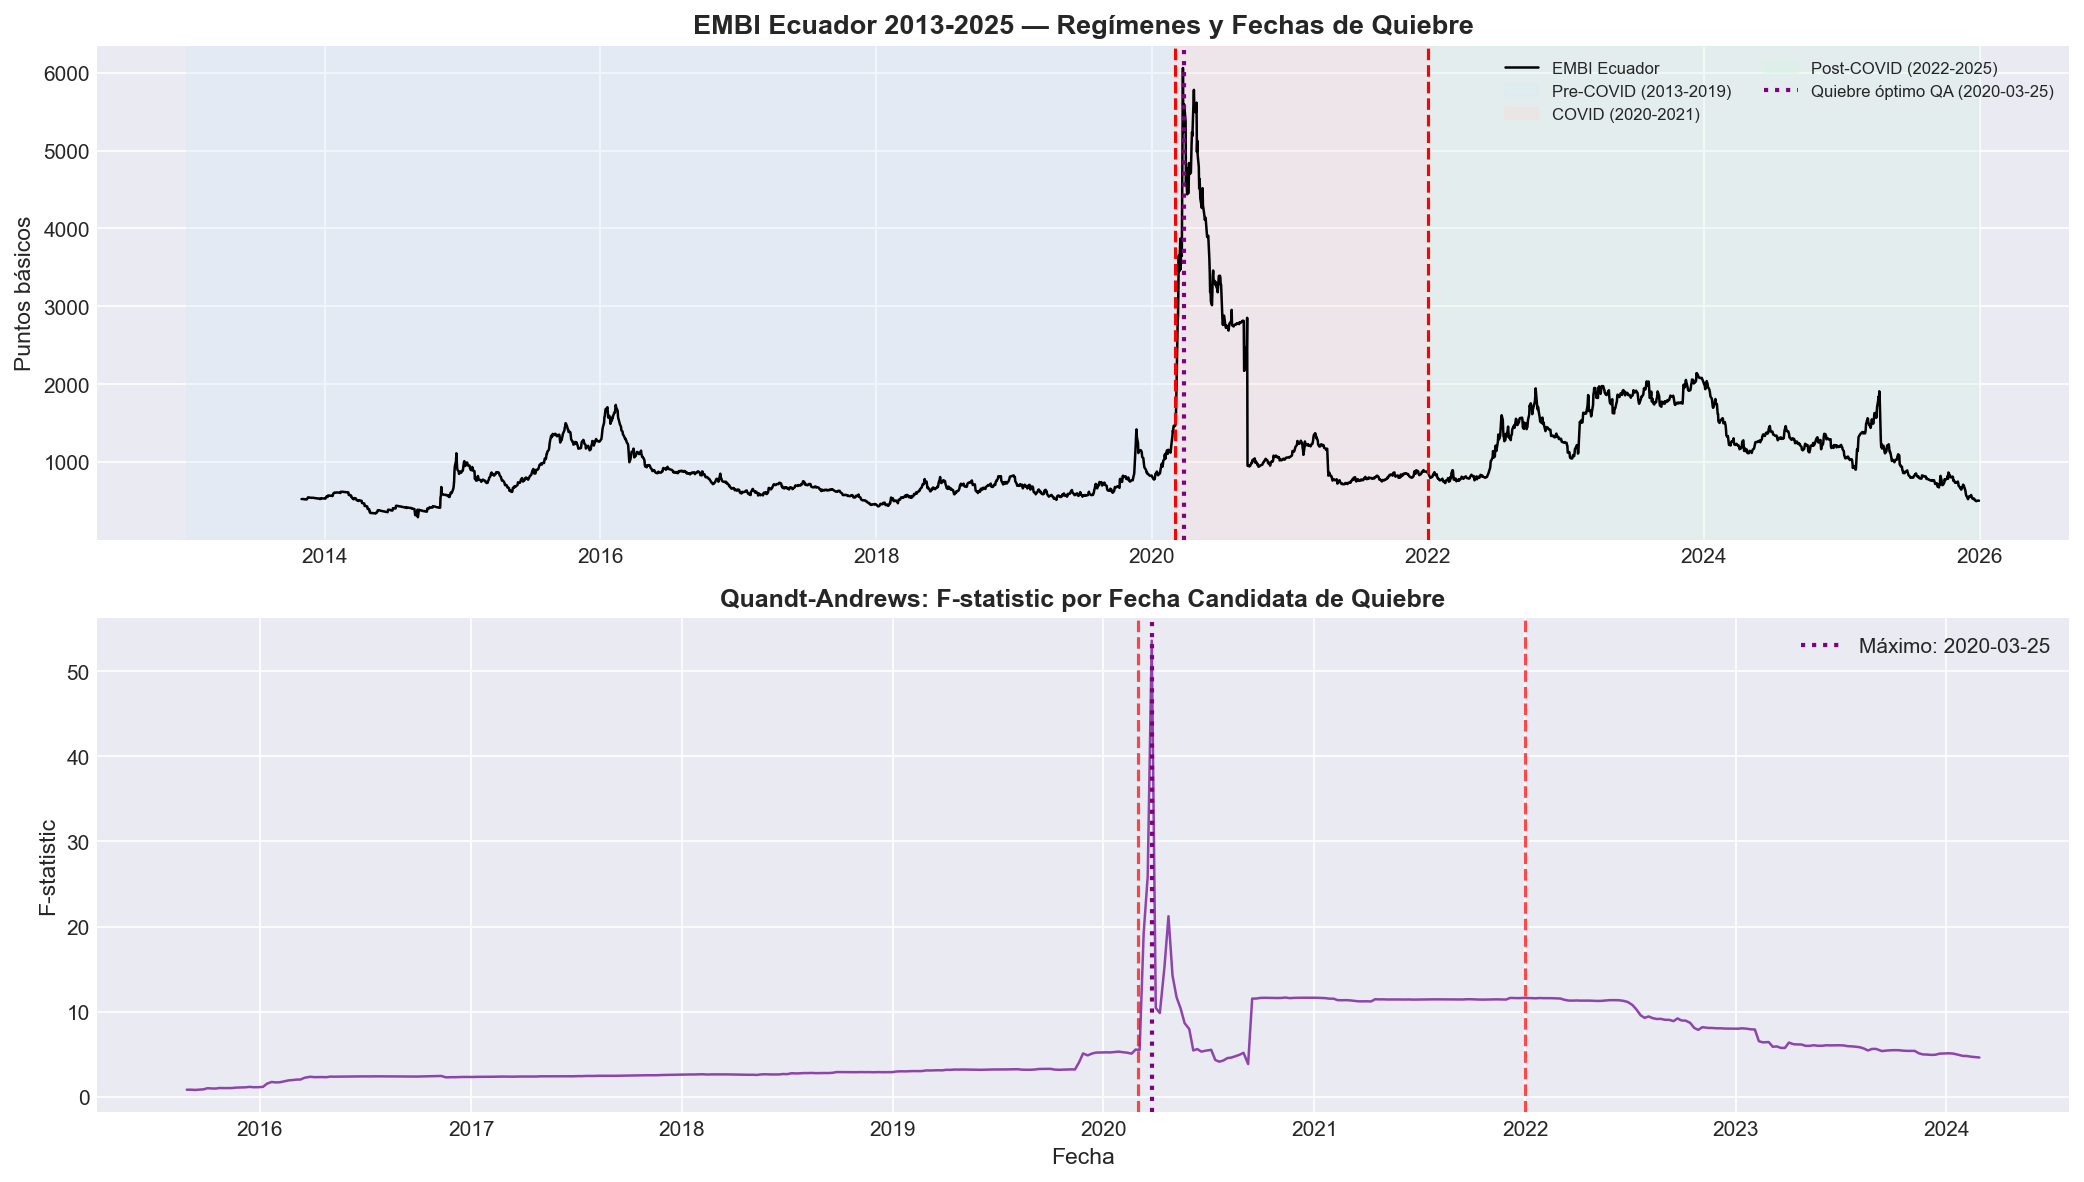
\includegraphics[width=0.85\textwidth]{chow_cusum_analysis.png}
\caption{CUSUM sobre residuos OLS AR(3) con bandas de confianza al 95\%}
\label{fig:cusum}
\end{figure}

\subsection{Importancia SHAP por régimen}

\begin{figure}[H]
\centering
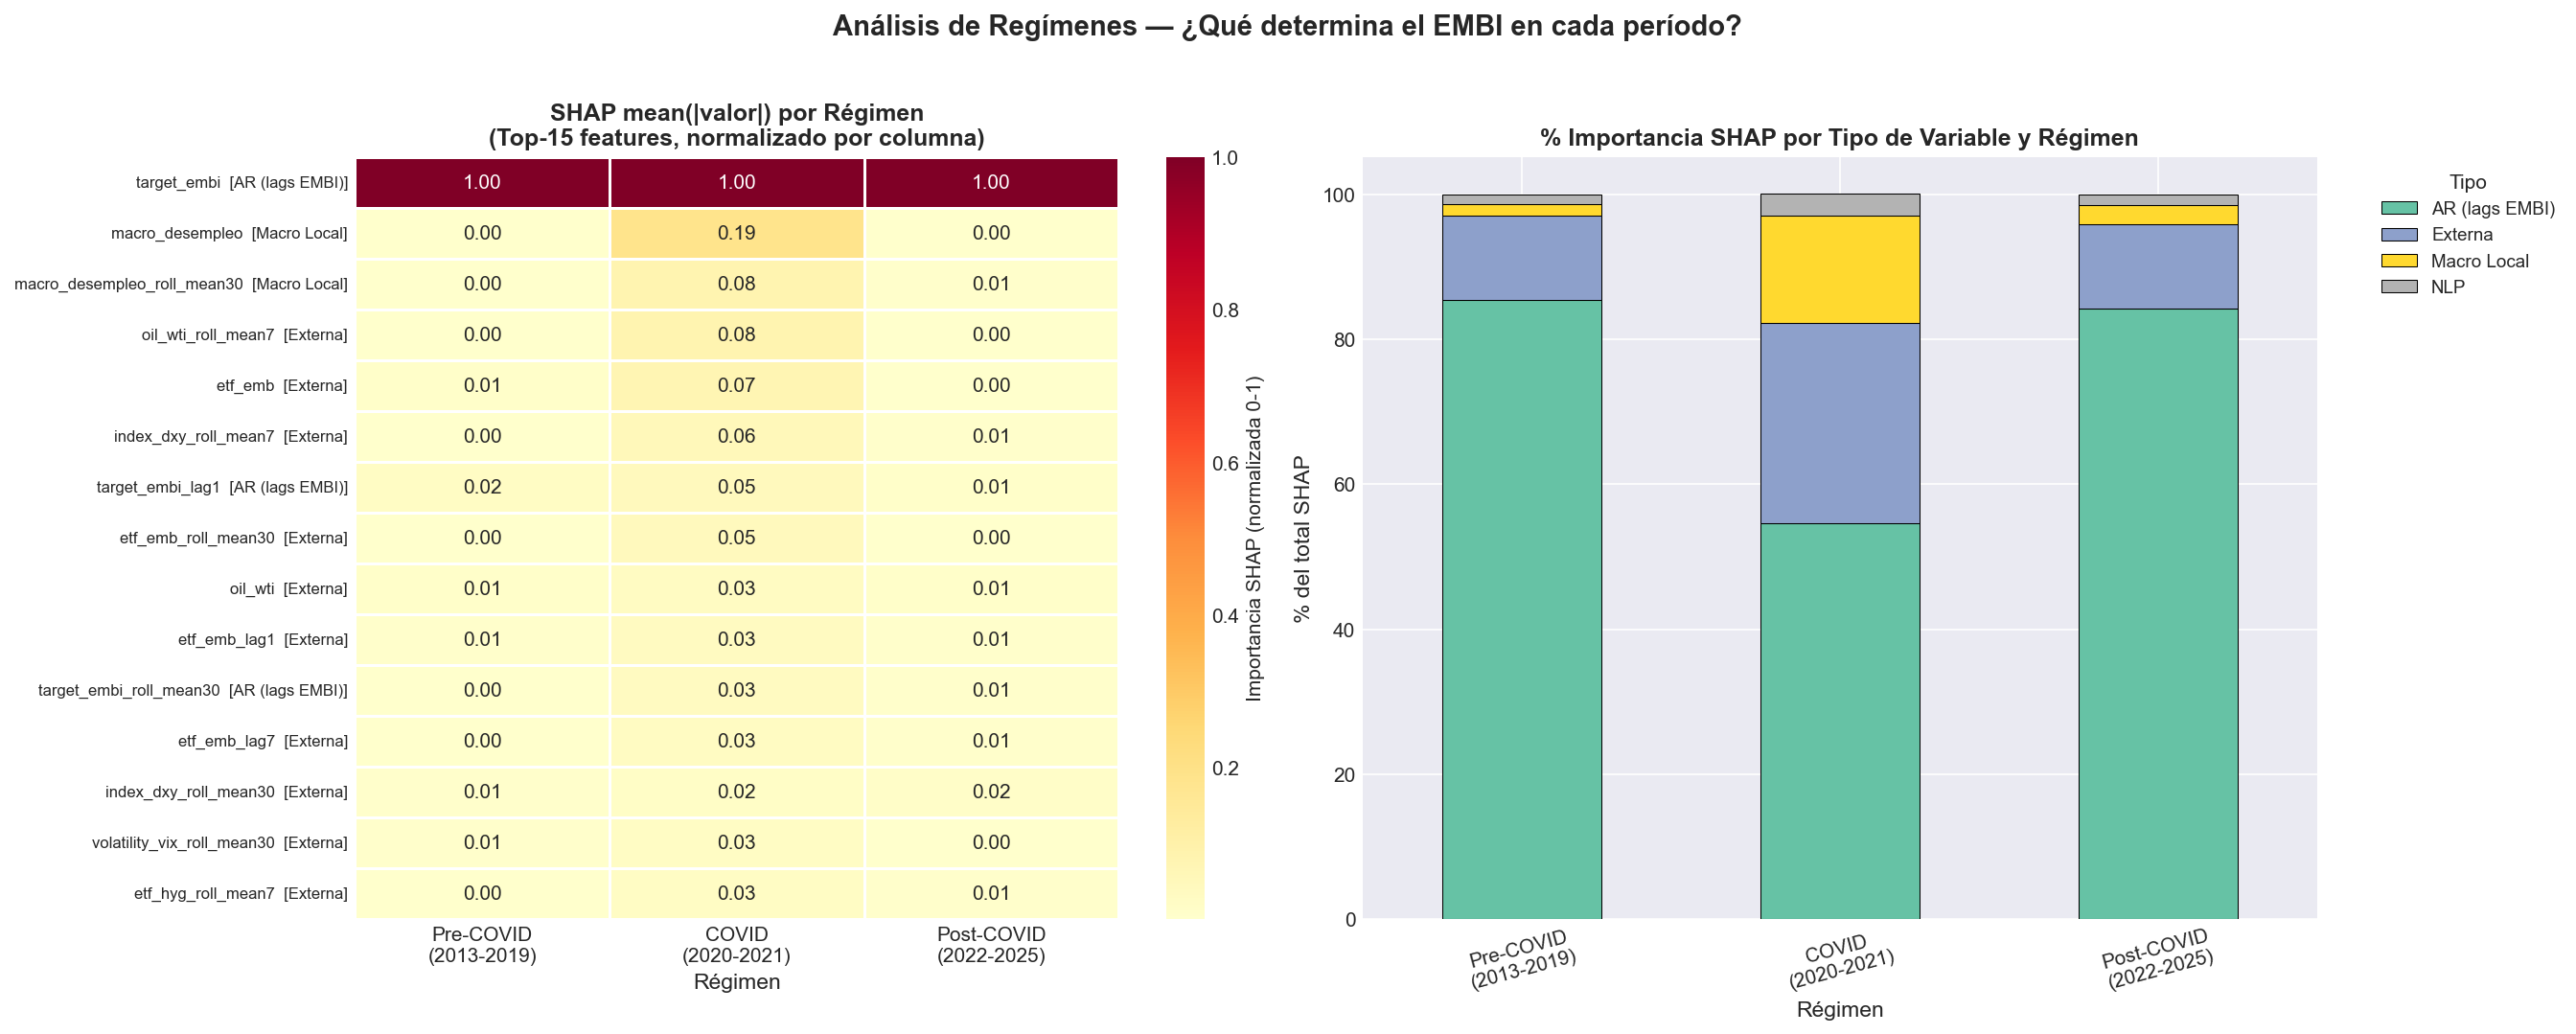
\includegraphics[width=\textwidth]{shap_regimenes_heatmap.png}
\caption{Heatmap de importancia SHAP (top-15 features) por régimen temporal}
\label{fig:shap_regimenes}
\end{figure}

\begin{figure}[H]
\centering
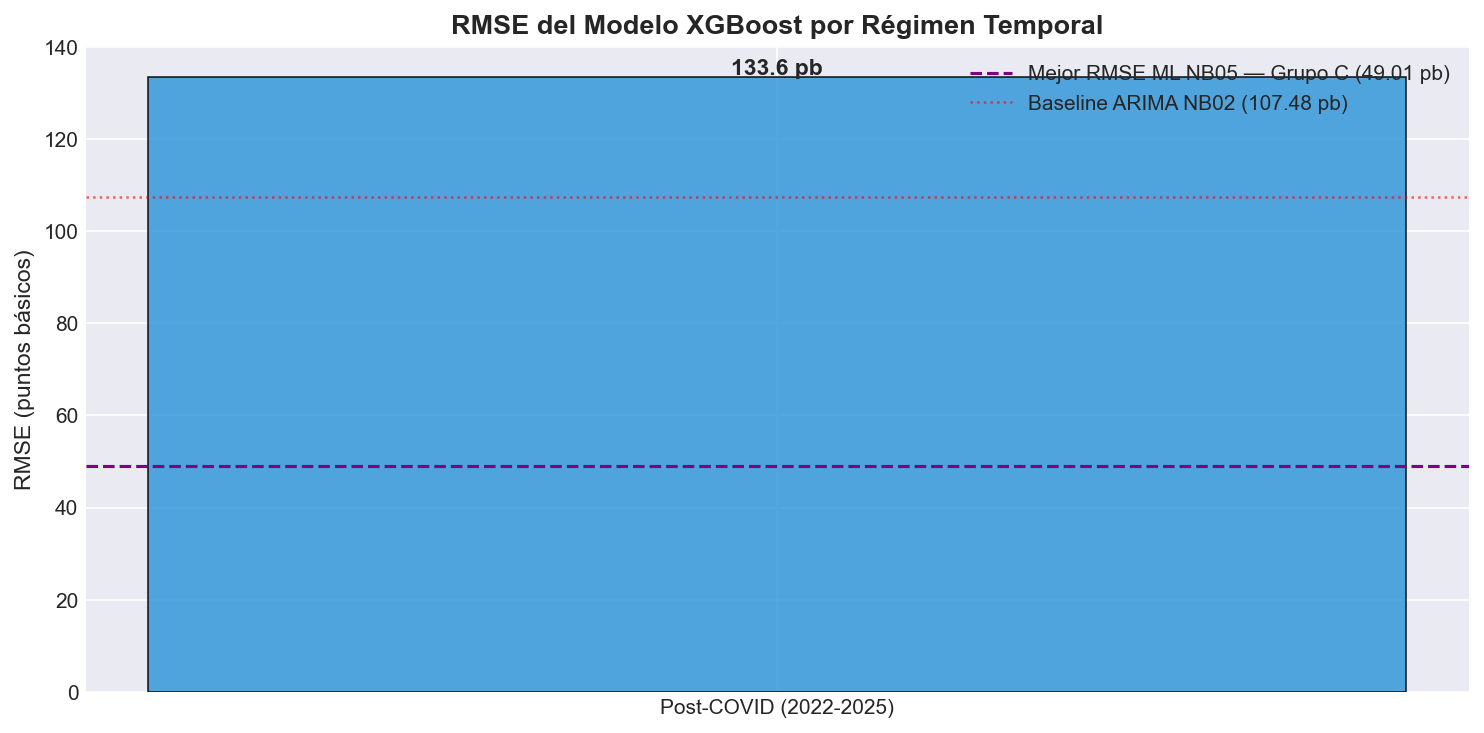
\includegraphics[width=0.75\textwidth]{rmse_por_regimen.png}
\caption{RMSE por subperíodo: pre-COVID, COVID, post-COVID}
\label{fig:rmse_regimen}
\end{figure}

% TODO: comentar los tres hallazgos del régimen:
%   1. Pre-COVID: exogeneidad total (variables externas + AR)
%   2. COVID: desempleo local irrumpe (SHAP=125.98)
%   3. Post-COVID: dominancia Fed + DXY en economía dolarizada

% --------------------------------------------------------
\section{Autoencoder NLP}
% --------------------------------------------------------

\begin{figure}[H]
\centering
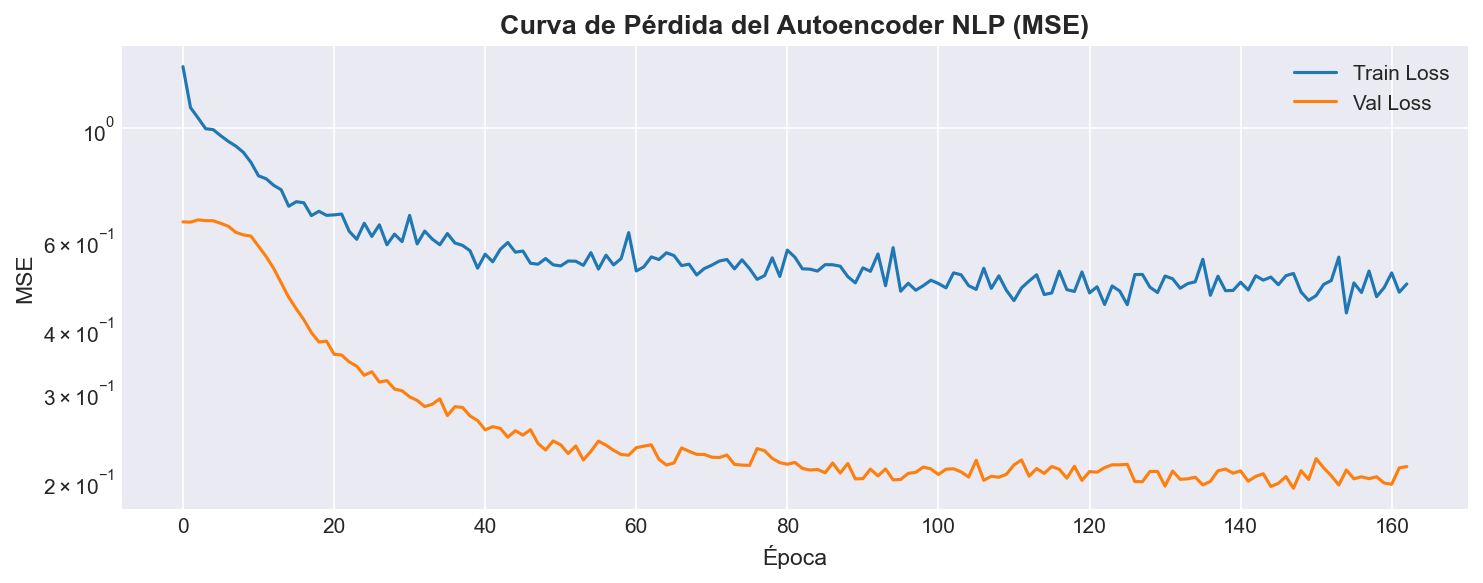
\includegraphics[width=0.7\textwidth]{autoencoder_loss_curve.png}
\caption{Curva de pérdida del autoencoder por época (train vs validación)}
\label{fig:ae_loss}
\end{figure}

\begin{table}[H]
\centering
\caption{Comparativa de representaciones NLP en el modelo XGBoost}
\label{tab:autoencoder}
\begin{tabular}{lcccc}
\toprule
\textbf{Representación NLP} & \textbf{Features} & \textbf{RMSE (pb)} & \textbf{MAE (pb)} & \textbf{R$^2$} \\
\midrule
Original (4 rolling 30d) & 4 & 59.29 & 39.37 & 0.9620 \\
PCA-3 (reducción lineal) & 3 & 60.11 & 41.14 & 0.9609 \\
Autoencoder-3 (no lineal)& 3 & 63.41 & 44.79 & 0.9565 \\
\bottomrule
\end{tabular}
\end{table}

\begin{figure}[H]
\centering
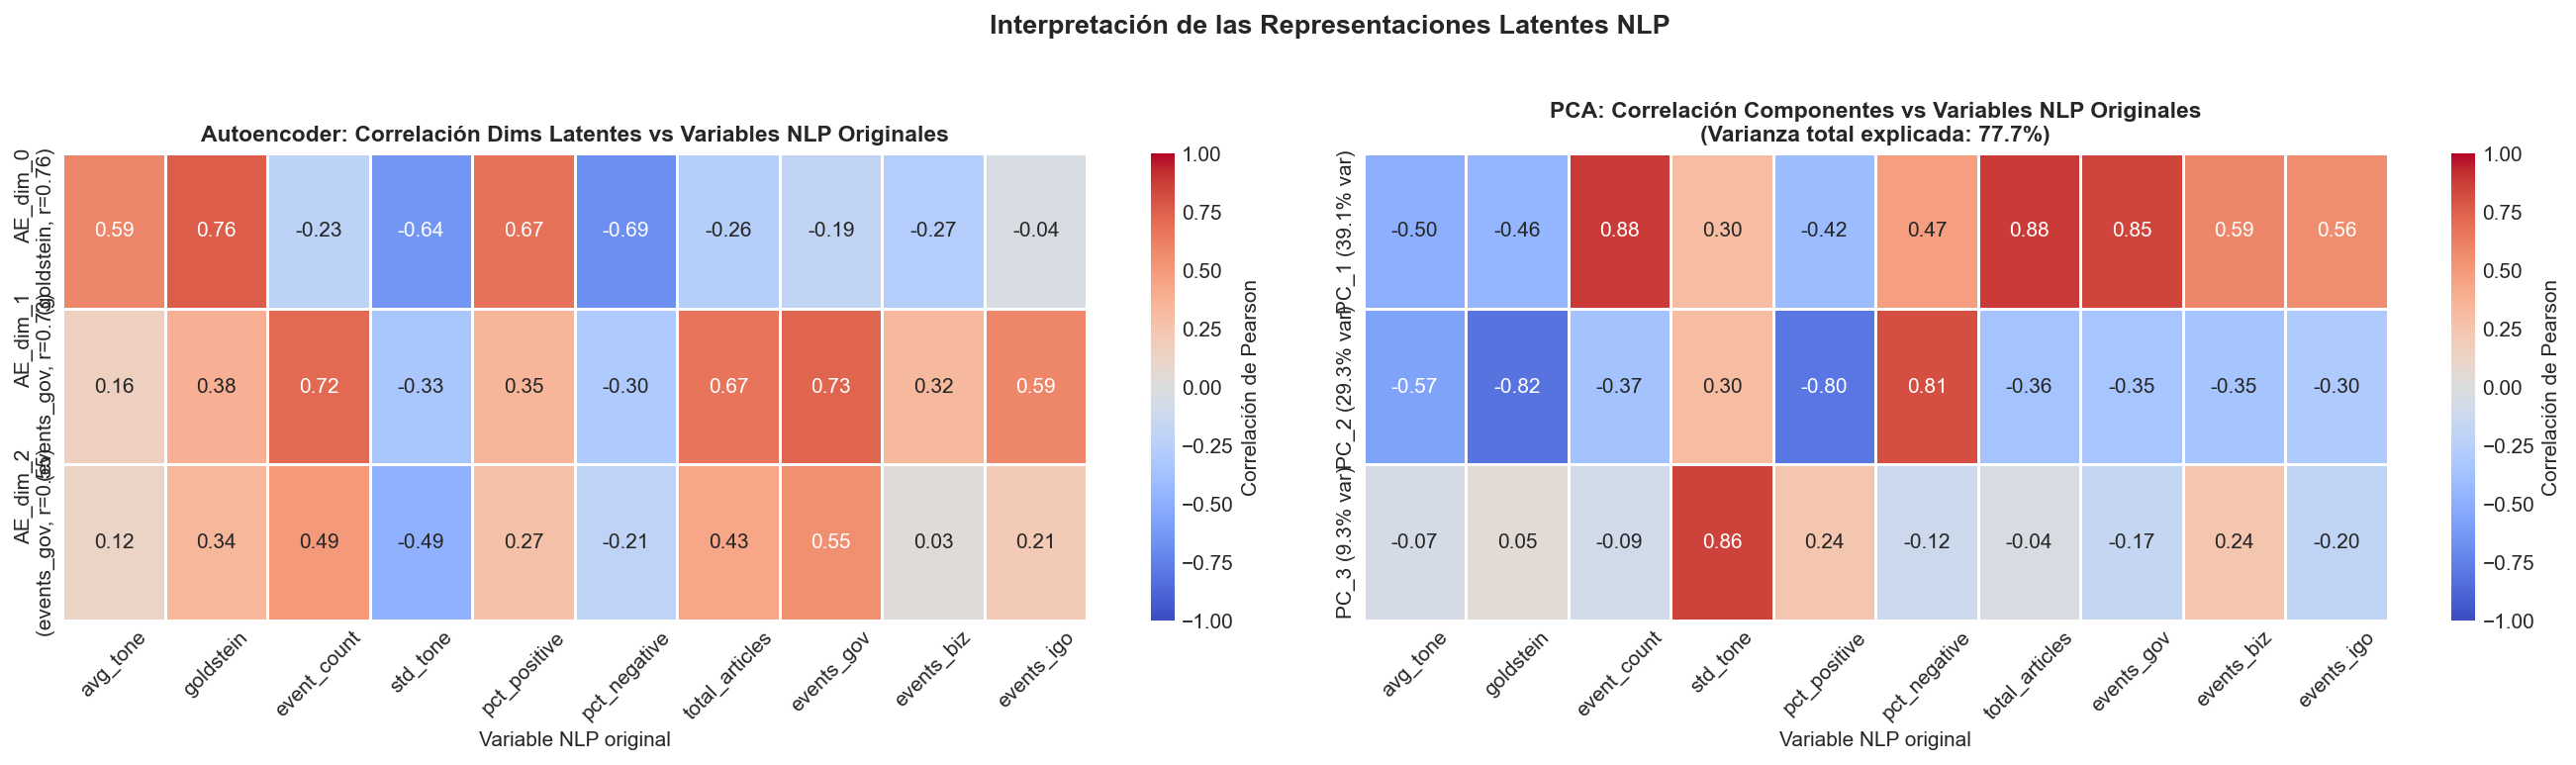
\includegraphics[width=0.75\textwidth]{nlp_latentes_correlacion.png}
\caption{Correlación entre dimensiones latentes del autoencoder y variables NLP originales}
\label{fig:ae_latentes}
\end{figure}

% TODO: comentar que la estructura NLP es esencialmente lineal (PCA 77.7% varianza en 3 comp)
% y que comprimir de 4→3 ya pierde señal predictiva marginal

\chapter{Discusión}

% --------------------------------------------------------
\section{¿El ML supera al ARIMA?}
% --------------------------------------------------------
% TODO: ~400 palabras
% - Sí, sustancialmente: 49-64 pb vs 107.48 pb (40-54% reducción)
% - El salto validación→test del ARIMA revela que no captura shocks exógenos
% - El XGBoost captura la persistencia AR + shocks contemporáneos del mercado
% - Relevancia económica: 1 pb EMBI ≈ X millones USD en costo de deuda

% --------------------------------------------------------
\section{¿El NLP agrega valor predictivo?}
% --------------------------------------------------------
% TODO: ~400 palabras
% - Sí: 2.30-2.59 pb de mejora incremental directa
% - El NLP que sobrevive feature selection es volumen (event_count, total_articles)
%   no sentimiento (avg_tone, goldstein eliminados)
% - Interpretación: el mercado reacciona a que "se hable de Ecuador" independientemente
%   del tono — incertidumbre mediática como proxy de riesgo
% - Granger negativo: la cobertura no anticipa, es contemporánea
% - Implicación: la relación NLP-EMBI no genera arbitraje temporal

% --------------------------------------------------------
\section{¿Es el EMBI ecuatoriano exógeno?}
% --------------------------------------------------------
% TODO: ~500 palabras — la sección más rica de la discusión
% - En períodos normales: sí (Pre-COVID: top features son EMBI lag + WTI + Treasury + ETF)
% - En crisis (COVID 2020): el desempleo local irrumpe como segundo factor (SHAP=125.98)
%   → el mercado evaluaba capacidad de pago local ante el default inminente
% - Post-COVID (2022-2025): Fed + DXY dominan absolutamente
%   → coherente con la dolarización: Ecuador no tiene política monetaria propia
% - Conectar con literatura: hipótesis de "sudden stops", Calvo et al.

% --------------------------------------------------------
\section{Contexto histórico: el default Correa 2008}
% --------------------------------------------------------
% TODO: ~300 palabras
% - En 2008-2009 Ecuador repudió ~$3.2B en deuda bajo Correa (bonos 2012 y 2030)
% - Decisión política, no fiscal — primer default voluntario moderno en AL
% - El EMBI llegó a 4.000+ pb durante el evento
% - Por qué no está modelado: GDELT v2 empieza en 2013; incluir GDELT v1 requeriría
%   reconciliar dos versiones con dimensiones distintas → trabajo futuro
% - Relevancia narrativa: confirma que Ecuador tiene régimen de riesgo propio
%   diferente al promedio EM

% --------------------------------------------------------
\section{Sobre la representación NLP: ¿lineal o no lineal?}
% --------------------------------------------------------
% TODO: ~300 palabras
% - Autoencoder no mejora sobre PCA (3.3 pb diferencia)
% - PCA captura 77.7% de varianza NLP en 3 componentes → estructura esencialmente lineal
% - Las 4 variables originales (rolling 30d) ya son una representación casi óptima
% - Implicación: para mejorar la señal NLP se necesitan datos de texto crudo
%   (embeddings BERT/FinBERT sobre noticias GDELT), no compresión de métricas agregadas

% --------------------------------------------------------
\section{Limitaciones}
% --------------------------------------------------------
% TODO: ~400 palabras
% 1. Dato diario vs frecuencia de publicación de variables macro (mensual/trimestral)
%    → solución: lags y rolling means, pero se pierde precisión intra-mes
% 2. GDELT como proxy mediático: no captura texto completo, solo eventos codificados
% 3. El período post-COVID (2024-2025) es atípico: reducción de EMBI 1.800→500 pb
%    bajo Noboa — posible "nuevo régimen" que el modelo histórico no captura bien
% 4. Ausencia de datos pre-2013 (GDELT v2) excluye el default 2008
% 5. El test de Wilcoxon con 5 folds tiene bajo poder estadístico

\chapter{Conclusiones y Trabajo Futuro}

% --------------------------------------------------------
\section{Conclusiones}
% --------------------------------------------------------
% TODO: ~400 palabras — responder directamente cada pregunta de investigación
%
% 1. Sí, el ML (XGBoost, Grupo C) supera al ARIMA: RMSE 49.01 vs 107.48 pb (reducción 54.4%)
%
% 2. El NLP aporta: 2.30-2.59 pb de mejora incremental. La señal es de volumen
%    de cobertura mediática, no de sentimiento.
%
% 3. Granger: el NLP no anticipa el EMBI con rezago. La relación es contemporánea;
%    el EMBI anticipa el tono de las noticias (no al revés).
%
% 4. Quiebres estructurales confirmados en 2020-03 y 2022-01. El EMBI ecuatoriano
%    es exógeno en períodos normales, parcialmente endógeno en crisis.
%
% 5. El autoencoder confirma que la representación NLP es esencialmente lineal —
%    resultado negativo informativo que guía trabajo futuro.

% --------------------------------------------------------
\section{Implicaciones para política económica}
% --------------------------------------------------------
% TODO: ~200 palabras
% - Un sistema de monitoreo del EMBI en tiempo real basado en este modelo
%   podría alertar al Ministerio de Finanzas sobre presiones de costo de deuda
% - La dominancia post-COVID del DXY y Treasury 10Y implica que la política
%   fiscal ecuatoriana tiene poco margen de acción sobre el EMBI en el corto plazo
% - El desempleo local como factor COVID sugiere que la credibilidad fiscal
%   interna sí importa en escenarios de estrés extremo

% --------------------------------------------------------
\section{Trabajo futuro}
% --------------------------------------------------------
% TODO: ~300 palabras — lista priorizada
%
% 1. LSTM end-to-end: red recurrente sobre secuencia completa (macro + NLP) — podría
%    capturar dependencias temporales de orden superior que XGBoost ignora
%
% 2. NLP con texto crudo: embeddings FinBERT sobre artículos de noticias GDELT
%    (requiere acceso a texto, no solo métricas agregadas). Hipótesis: el sentimiento
%    del texto crudo sí anticipa el EMBI cuando el tono agregado no lo hace
%
% 3. Extender a 2008 con GDELT v1: incluir el default Correa requiere reconciliar
%    dos versiones del dataset con dimensiones diferentes
%
% 4. Modelos por régimen: entrenar XGBoost separado para cada subperiodo (pre-COVID,
%    COVID, post-COVID) y comparar con el modelo global
%
% 5. Panel de países EM: extender el análisis a Ecuador + Colombia + Perú + Argentina
%    para identificar qué factores son idiosincráticos de Ecuador vs regionales


% --- Bibliografía ---
\printbibliography[heading=bibintoc, title={Referencias}]

% --- Anexos ---
\appendix
\chapter{Anexos}

% --------------------------------------------------------
\section{Hiperparámetros óptimos del XGBoost}
% --------------------------------------------------------
% TODO: tabla completa con todos los hiperparámetros del RandomizedSearchCV

% --------------------------------------------------------
\section{Variables del dataset completo}
% --------------------------------------------------------
% TODO: tabla con las 22 variables originales, fuente, frecuencia, período

% --------------------------------------------------------
\section{Los 60 features seleccionados por Mutual Information}
% --------------------------------------------------------
% TODO: tabla completa con nombre, categoría, score MI

% --------------------------------------------------------
\section{Resultados completos de causalidad de Granger}
% --------------------------------------------------------
% TODO: tabla completa con todos los pares y lags testados

% --------------------------------------------------------
\section{Arquitectura del autoencoder}
% --------------------------------------------------------
% TODO: diagrama o tabla de capas con parámetros


\end{document}
